\section{Entwicklung der neuen Benutzeroberfläche für Vermögensauskünfte}
Eine Hauptaufgabe des Projektes ist der Entwurf und die Implementierung einer neuen grafischen Benutzerschnittstelle für die Eingabe von Vermögensverzeichnissen. Diese neue Benutzeroberlfäche soll später die bestehende Eingabeschnittstelle für Vermögensverzeichnisse ablösen. Die neue Eingabemaske soll sich an den Gestaltungsgesetzen, Normen, Verordnungen und Usability Heuristiken, die in den Kapiteln 4.2.2, 4.2.3, 4.2.4 und 4.2.5 vorgestellt wurden, orientieren und die darin enthaltenen Empfehlungen und Prinzipien berücksichtigen. Ebenso erfolgt der Entwicklungsprozess in Anlehnung an das Vorgehensmodell aus Kapitel 4.4. Für die initiale Projektvorstellung meiner Bachelor Thesis, wurden im Vorhinein bereits mehrere fachlich und technisch visierte Ansprechpartner mit einbezogen. Während des Entwicklungsprozesses wurden mehrere Gespräche sowohl mit den fachlichen Anforderungsstellern als auch mit den technischen Beteiligten geführt, um die Anforderungen für den neuen Dialog möglichst genau zu definieren.

%%%%%%%%%%%%%%%%%%%%%%%%%%%%%%%%%%%%%%%%%%%%%%%%%%%%%%%%%%%%%%%%%%%%%%%%%%%%

\subsection{Vorgehensmodell für den Entwicklungsprozess}

Zunächst wird das Vorgehensmodell nach ISO 9241-210 an den zeitlichen Rahmen und den Inhalt meines Projektes angepasst. Das Ziel der neuen Benutzeroberfläche ist es möglichst benutzerfreundlich und individuell auf die Benutzer und deren Arbeitsabläufe abgestimmt zu sein. Dafür eignet sich das Usability-Engineering als agiles Modell gut. Insbesondere da eine möglichst benutzerorientierte Aufnahme der Anforderungen und Wünsche erfolgen soll. Zudem soll auch ein iteratives Testvorgehen angewandt werden. Das heißt, dass nach jeder entwickelten Gestaltungslösung Benutzungstests von zwei bis drei Testern durchgeführt werden. Die Prototypen werden auf einer separaten Entwicklungsumgebung getestet. Bei den Tests prüfen die Tester den Prototypen auf fachliche und technische Fehler, damit die Wahrscheinlichkeit für schwerwiegende Systemfehler (Systemabsturz, Speicherprobleme o.Ä.) möglichst gering gehalten wird. Die Sachbearbeiter sollen nämlich beim anschließenden Produktivtest reibungslos Arbeiten können. Systemfehler würden sich in den erhobenen Daten widerspiegeln und schlimmsten falls zu Auswertungsfehlern bzw. einem größeren Aufwand für die Fehlerbehebung führen.

Solange die Gestaltungslösungen die Erwartungen und Anforderungen nicht erfüllen kann iterativ in vorherige Phasen gesprungen werden. Sobald ein finaler Entwicklungsstand vorliegt, wird dieser in die produktiv Umgebung ausgerollt, damit anschließend die Evaluation inklusive empirischer Erhebung, zum neuen Dialog, stattfinden kann.

%%%%%%%%%%%%%%%%%%%%%%%%%%%%%%%%%%%%%%%%%%%%%%%%%%%%%%%%%%%%%%%%%%%%%%%%%%%%

\subsection{Aufnahme des Ist-Zustands}
Die Aufnahme des Ist-Zustands ist mit den ersten beiden Phasen des ISO 9241-210 Vorgehensmodell zu vergleichen. Dazu gehört die Erhebung des Nutzungskontextes (Benutzergruppen, Arbeitsabläufe und technisches Umfeld) und der Anforderungen. Da man sich in dem Projekt dazu entschieden hat eine bestehende Eingabeoberfläche durch eine komplett neue  auszutauschen, eignet sich die bestehende sehr gut als Grundlage für die Anforderungsanalyse. Die Beurteilung von Schwächen und Stärken der aktuellen Benutzerschnittstelle hilft dabei gezielte Anforderungen für den neuen Dialog zu schaffen.

%%%%%%%%%%%%%%%%%%%%%%%%%%%%%%%%%%%%%%%%%%%%%%%%%%%%%%%%%%%%%%%%%%%%%%%%%%%%

\subsubsection{Benutzergruppen}
Zunächst werden die Benutzergruppen und -typen, die später mit der neuen Schnittstelle interagieren, genauer analysiert. Mit Hilfe eines Fragebogens werden das Alter, das Geschlecht, die wöchentlich durchschnittliche Nutzungsdauer von Computern allgemein sowie die der Eingabeoberfläche für Vermögensverzeichnisse ermittelt. Das durchschnittliche Benutzerprofil wurde auf der Basis von ?? Benutzern aufgestellt und ist in Abbildung \ref{fig:durchschnittlichesBenutzerprofil} abgebildet. 

Die Abteilung wurde aufgrund der vielen unterschiedlichen Ausprägungen im durchschnittlichen Benutzerprofil nicht berücksichtigt. Da es sich bei dem Geschlecht nur um ein nominal skaliertes Merkmal handelt, wurde als Referenzwert der Modalwert ermittelt. Die anderen drei Merkmale sind alle metrisch (gehören zur Kardinalskala), daher konnten die Referenzwerte mit Hilfe des arithmetischen Mittels berechnet werden.
\begin{figure}[H]
  \centering
  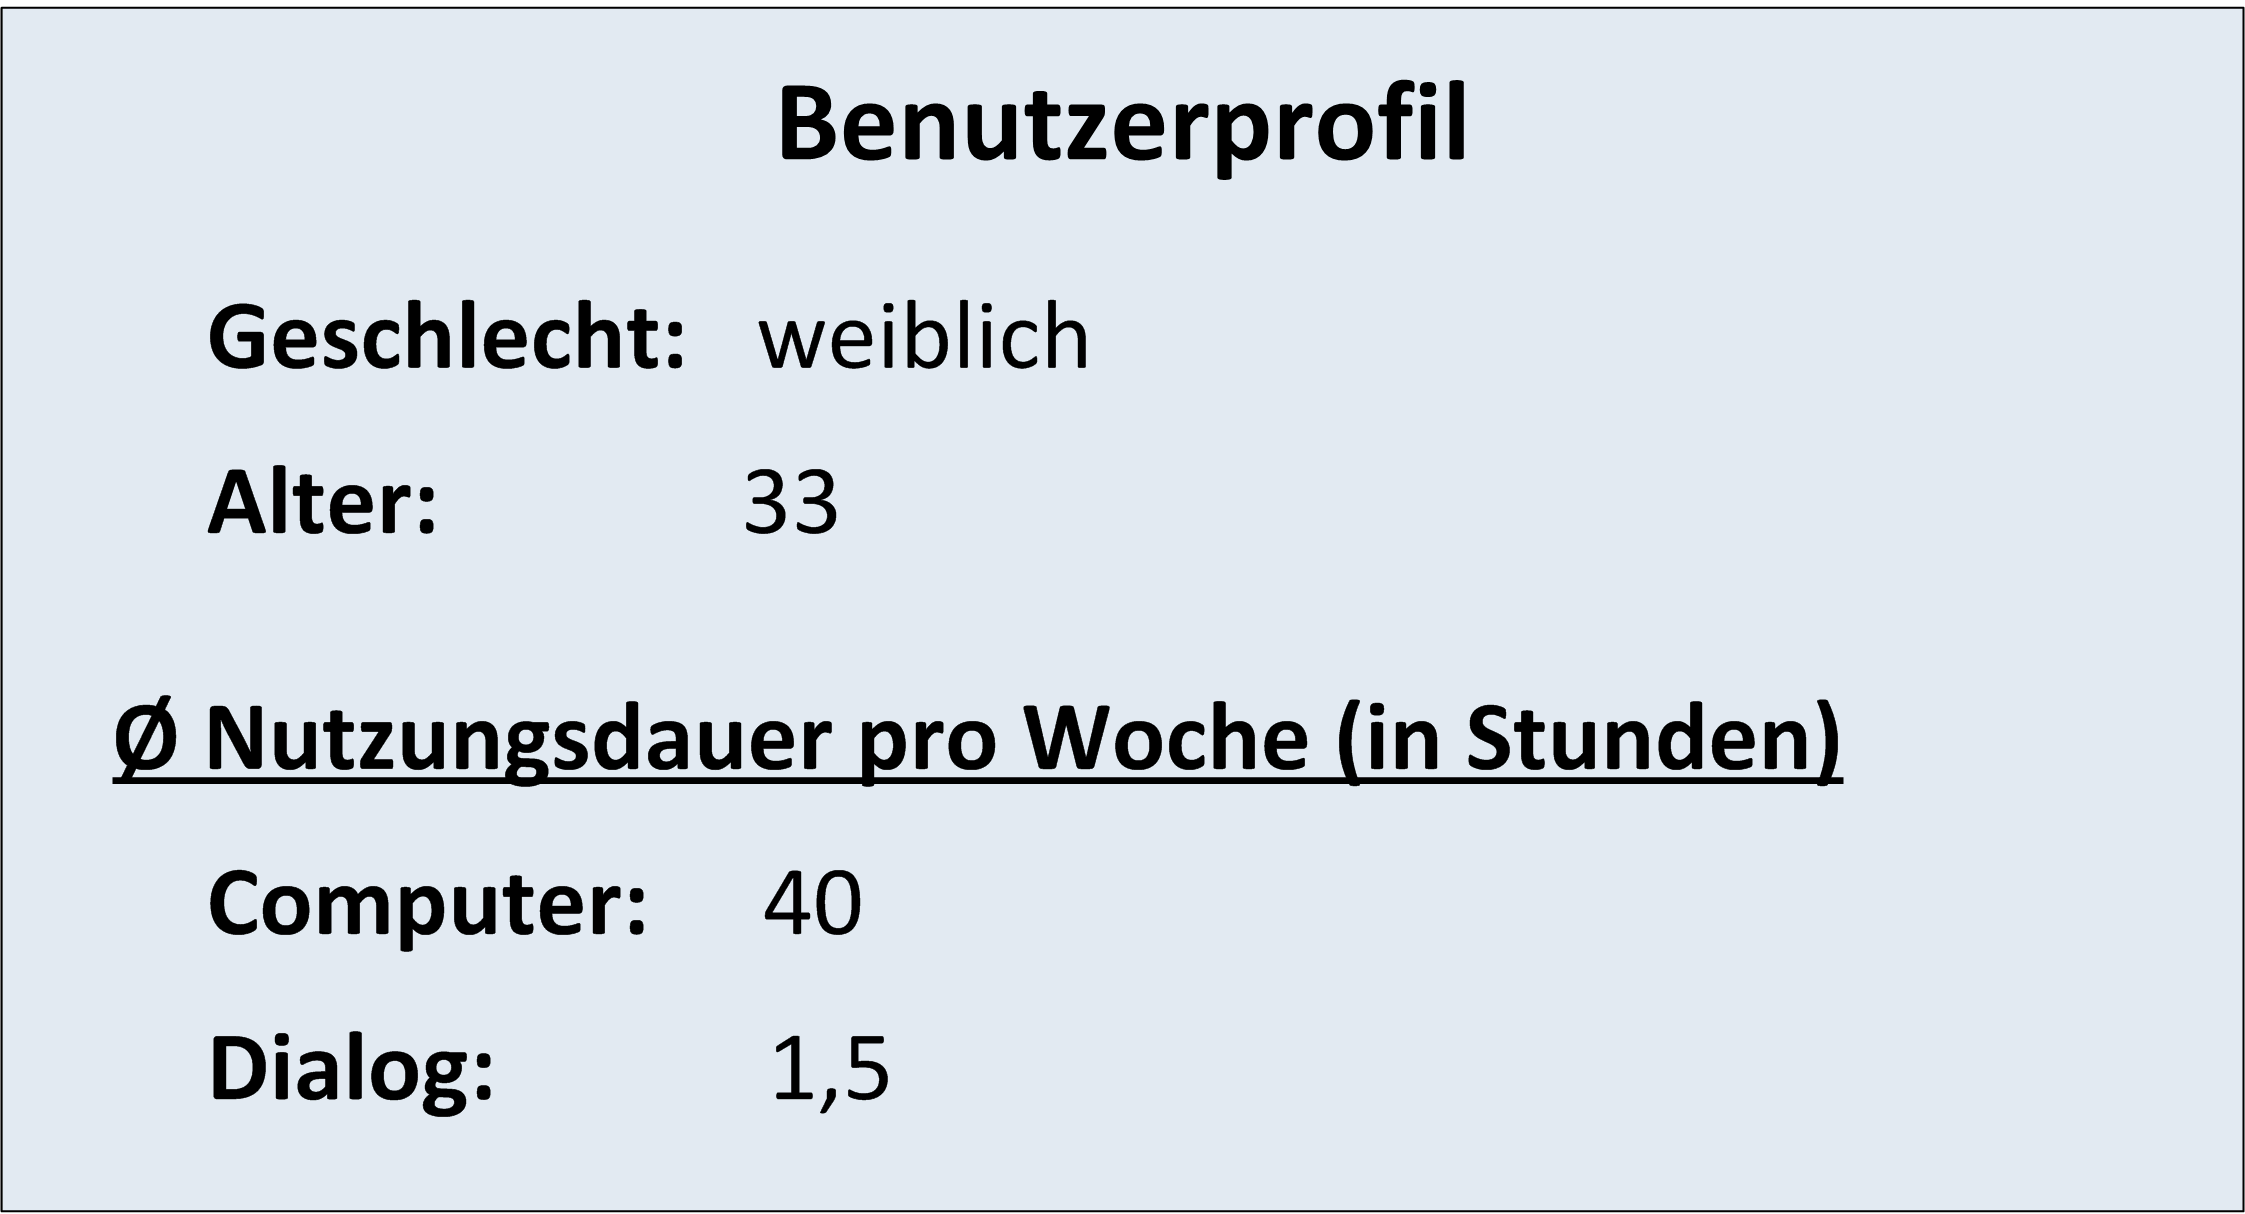
\includegraphics[width=295px]{img/durchschnittliches_Benutzerprofil.png}
  \caption{Durchschnittliches Benutzerprofil.}
  \caption*{\textbf{Quelle:} eigene Darstellung}
  \label{fig:durchschnittlichesBenutzerprofil}
\end{figure}
Es lässt sich feststellen, dass sich größtenteils Frauen in der Sachbearbeitung befinden. Zudem ist das durchschnittliche Alter der Benutzer auf rund ?? Jahre zu schätzen. Trotzdem sollte darauf Rücksicht genommen werden, dass der maximale Altersunterschied bei ?? Jahren liegt. Die Benutzergruppe setzt sich sowohl aus sehr jungen, als auch aus kurz vor der Rente stehenden Sachbearbeitern zusammen. Dies kann besonders bei der Erfahrung wie auch bei der Lernfähigkeit und Lernbereitschaft zu Diskrepanzen führen.

Betrachtet man die durchschnittliche Nutzungsdauer des Computers von ?? Stunden, so ist zu erkennen, dass die Sachbearbeiter großenteils mit dem PC arbeiten und daher mit dem generellen System vertraut sein sollten. Anders sieht es bei Nutzung des Eingabedialogs für Vermögensverzeichnisse aus. Durchschnittlich arbeiten die Benutzer ?? Stunden mit dem Dialog. Jedoch herrschen hier relativ große Unterschiede bei der Nutzungsdauer, die durch die unterschiedlichen Mandanten und Aufgabenbereiche der Teams zu begründen sind. Manche Teams müssen sehr häufig den Anwendungsfall \glqq Eingabe eines Vermögensantrags\grqq{} behandeln andere nur eher selten. Daher ist davon auszugehen, das auch die Effizienz bei der Benutzung, auf unterschiedlichen Niveaus sein wird. Dies sollte man bei der Evaluation und Datenauswertung im Anschluss ebenfalls berücksichtigen.

%%%%%%%%%%%%%%%%%%%%%%%%%%%%%%%%%%%%%%%%%%%%%%%%%%%%%%%%%%%%%%%%%%%%%%%%%%%%

\subsubsection{Arbeitsabläufe und Tätigkeiten}
Die Arbeitsabläufe wurden mit Hilfe eines persönlichen Interviews und einer Analyse der bestehenden Schnittstelle entworfen und modelliert. Dabei wurde zum einen der Ablauf einer  Zwangsvollstreckung im Ganzen dargestellt (siehe Anhang \ref{sec:ablaufZwangsvollstreckung}) und zum anderen der Arbeitsprozess eines einzelnen Mitarbeiters bei der Eingabe des Vermögensverzeichnisses in das System.

%%%%%%%%%%%%%%%%%%%%%%%%%%%%%%%%%%%%%%%%%%%%%%%%%%%%%%%%%%%%%%%%%%%%%%%%%%%%

\subsubsection{Technisches Umfeld}
Für die Aufnahme des technischen Umfelds wurde sich mit den Beteiligten des Projekts für ein offenes Interview (siehe Kap. 4.3.3) entschieden. Dabei ist herausgekommen, dass alle Sachbearbeiter standardmäßig mit zwei Monitore und dem Betriebssystem Windows ausgestattet sind. Darüber hinaus stehen den Sachbearbeitern jeweils Maus und Tastatur als weitere Peripherie zur Verfügung. Hilfsmittel wie Drucker sind verteilt vorhanden, werden aber für den vorliegenden Anwendungsfall nicht benötigt, da das Vermögensverzeichnis Dokument in digitaler Form vorliegt. Die weitere Ausstattung für einen Sachbearbeiter sieht einen eigenen Arbeitsplatz vor, der sich je nach Team und Abteilung unterscheiden kann. Typischerweise befinden sich Trennwände zwischen den einzelnen Arbeitsplätzen, um gerade in Großraumbüros die Akustik und Arbeitsatmosphäre zu verbessern. Zusammengefasst ist die Ausstattung und das Umfeld der Sachbearbeiter stark standardisiert und bietet damit für Jeden eine ähnliche Ausgangslage bei der Bearbeitung.

%%%%%%%%%%%%%%%%%%%%%%%%%%%%%%%%%%%%%%%%%%%%%%%%%%%%%%%%%%%%%%%%%%%%%%%%%%%%

\subsubsection{Anforderungsanalyse}
Zunächst wurde in einem initialen Termin darüber gesprochen welche grundsätzlichen Veränderungen die neue Oberfläche im Gegensatz zu der bestehenden Maske mit sich bringen soll. Dafür wurde gemeinsam mit den Beteiligten des Projekts der aktuelle Ist-Zustand der Oberfläche aufgenommen. Die Benutzeroberfläche in Abbildung \ref{fig:aktuellerDialog} ist aktuell produktiv im Einsatz. Diese wurde analysiert und es wurden sowohl negative als auch positive Aspekte aufgegriffen und entsprechende Design Anforderungen für die neue Oberfläche herausgearbeitet.
\begin{figure}[H]
  \centering
  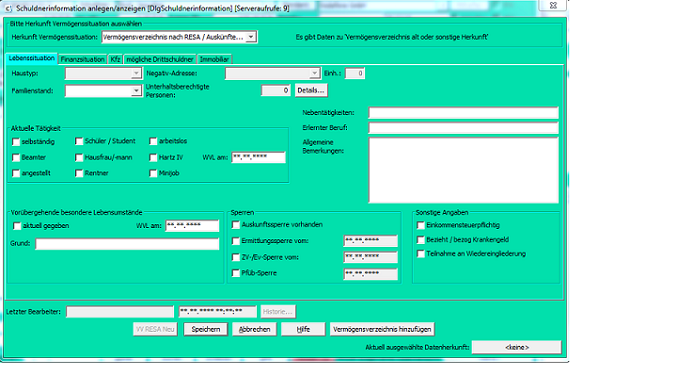
\includegraphics[scale=1]{img/aktueller_Dialog.PNG}
  \caption{Aktueller Dialog für die Eingabe von Vermögensverzeichnissen.}
  \caption*{\textbf{Quelle:} Vermögensverzeichnis Dialog der IFM}
  \label{fig:aktuellerDialog}
\end{figure}

Gleich zu Anfang wurde zusammen mit dem zuständigen Fachbereich definiert, welche Bedienelemente in der aktuellen Oberfläche nicht benötigt werden und für die neue Oberfläche somit wegfallen können. Als Ergebnis stellten sich drei grundlegende Gestaltungsziele heraus. Zu diesen Zielen gehören eine übersichtlichere Anordnung der Bedienelemente, eine reduzierte Auswahl an Bedienelementen mit der Prämisse das die benötigen Elemente zur Verfügung stehen und eine an das Vermögensverzeichnis angelehnte Struktur der Eingabeelemente. Zudem wurde für den Entwurf des Prototypen entschieden, dass die Datenstruktur vorerst bestehen bleiben sollte und Änderungen an dieser erst in einem nachfolgenden Projekt umgesetzt werden sollen.

Mit dieser Ausgangssituation an Zielen wird der erste fertig programmierte Prototyp für die Oberfläche entworfen. Dieser wird den Beteiligten dann in einem weiteren Termin präsentiert und anschließend auf einer Testumgebung zur Verfügung gestellt.

%%%%%%%%%%%%%%%%%%%%%%%%%%%%%%%%%%%%%%%%%%%%%%%%%%%%%%%%%%%%%%%%%%%%%%%%%%%%

\subsection{Erarbeitung der Gestaltungslösung}
Im folgenden wird genauer auf den Entwurfsprozess inklusive der Analysemethoden (siehe Kap. \ref{sec:analysemethoden}) genauer eingegangen. Dieser Teil des Entwicklungsprozesses ist mit den Phasen drei und vier aus dem ISO 9241-210 Vorgehensmodell (siehe Kap. 4.4.1) zu vergleichen. Das nachfolgende Vorgehen orientiert sich ebenfalls an dem iterativen Ansatz, bei dem besonderes die Phasen zwei, drei und vier mehrmals durchlaufen wurden, bis die fertige Lösung bereit stand. Die Gestaltungslösungen wurden dabei mit Hilfe von Interviews und heuristische Evaluationen bewertet und evaluiert.

\textbf{Erster Prototyp}

Der erste Prototyp wurde aufgrund der Anforderungen bewusst nur auf die benötigten Bedienelemente reduziert und sollte mit seiner Formular nahen Struktur einen klaren Fortschritt im Bereich der Übersichtlichkeit verzeichnen. Ebenfalls ist speziell durch die Berücksichtigung der Gestaltgesetze zur Ähnlichkeit und Nähe von Objekten eine klarere Unterteilung von Bedienelementgruppen entstanden. Dies hat die positive Folge das thematisch bzw. strukturell, durch das Formular, nah beieinander liegende Informationen deutlicher werden. Ebenso wurde auf einheitlich, verständlich und präzise formulierte Fehler- und Hinweismeldungen Wert gelegt. Auch hier kamen wieder die Empfehlungen der ISO Norm 9241-110 und die Heuristiken von Jakob Nielsen zu Gute. Durch die Vorgaben der Styleguides musste zudem auf eine entsprechende Dimensionierung von Elementen, so wie auf uneingeschränkte Vergrößerung der Anzeige geachtet werden.

Durch den zweiten Termin in dem der erste Prototyp präsentiert und anschließend evaluiert wurde, konnten die Beteiligten erstmals Eindrücke zu der neuen Oberfläche gewinnen. Zudem konnten erste Benutzungstest auf einer Entwicklungsumgebung durchgeführt werden. Aus der Präsentationsrunde sowie den Benutzungstests gingen überwiegend positive Rückmeldungen zu dem ersten Entwurf hervor. Jedoch war die Auswahl sowie Platzierung gewisser Bedienelemente noch nicht vollständig zufriedenstellend. 

Aufgrund der festgestellten Mängel wurde noch mal in die Anforderungsanalyse gesprungen, um die Anforderungsliste zu verfeinern und mit konkreten Verbesserungsvorschlägen zu bestücken. Diese erweiterten Anforderungen sollten anschließend in einer erneuten Konzeptionsphase durch einen zweiten Prototypen umgesetzt werden.

\textbf{Finale Version}

Mit Abschluss des ersten Prototypen und der erweiterten Anforderungsliste die aus der Analyse der Stärken und Schwächen resultierte, wurde ein weiterer Prototyp konzipiert. Der in Abbildung \ref{fig:neuerDialog} zu sehende Prototyp ist in drei Sektionen gegliedert, die durch die Verwendung von Rahmenlinien hervorgehoben werden. 
\begin{figure}[H]
  \centering
  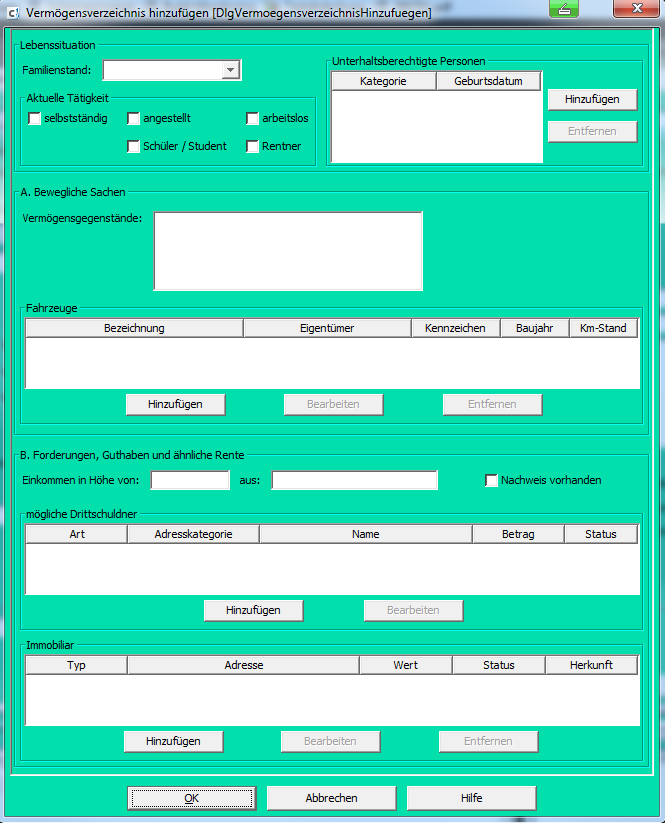
\includegraphics[scale=0.85]{img/neuer_Dialog.PNG}
  \caption{neuer Dialog für die Eingabe von Vermögensverzeichnissen.}
    \caption*{\textbf{Quelle:} eigene Darstellung}
  \label{fig:neuerDialog}
\end{figure}
Die erste Sektion beinhaltet Informationen zur allgemeinen Lebenssituation eines Schuldners, darunter zum Beispiel der Familienstand oder auch die Art der Tätigkeit. Ein weiteres Unterziel für die neue Oberfläche war es die Bezeichnungen von Eingabfeldern, Dropdownlisten, Buttons und Checkboxen soweit es geht beizubehalten. Der Nutzen daraus soll später durch eine schnellere Gewöhnung an die neue Oberfläche ersichtlich werden. Durch gleichnamige Felderbezeichnungen werden die Sachbearbeiter an alte bekannte Strukturen erinnert, die sie bereits kennen und brauchen dadurch bestenfalls weniger Einarbeitungszeit.

Die zweite Sektion des Dialogs visualisiert alle beweglichen Daten. Die Formulierung \glqq bewegliche Daten\grqq{} wurde aus dem standardisierten Formular übernommen und enthält Daten zu Vermögensgegenständen und Fahrzeugen der Schuldner. Eine grundlegende Veränderungen wurde bei der Eingabe von Fahrzeugen vorgenommen. Die Informationen zum Fahrzeug wurden zuvor in einzelnen Textfeldern (Bezeichnung, Eigentümer, Kennzeichen u.a.) eingetragen. Diese Textfelder standen aber nur einmal zur Verfügung. Sobald mehr als ein Fahrzeug hinterlegt wurde, mussten die Informationen in einem freien Textfeld \glqq weitere Fahrzeuge\grqq{} \ref{fig:fahrzeugTab} eingetragen werden. Diese Lösung war zum einen unschön, da es eine inkonsistente Eingabe gleicher Daten gab und zum anderen auch fehleranfällig, weil einzutragende Informationen schneller vergessen wurden. 
\begin{figure}[H]
  \centering
  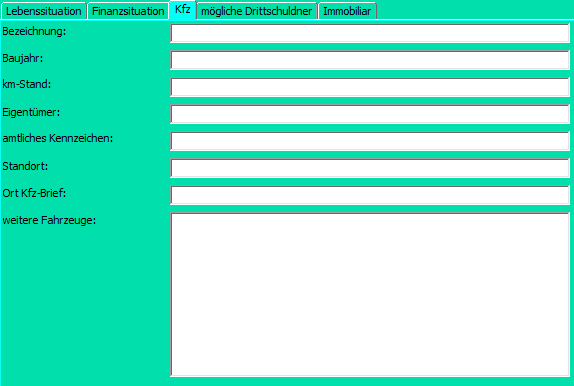
\includegraphics[scale=0.9]{img/FahrzeugTab.PNG}
  \caption{Eingabemaske für Fahrzeuge in der alten Oberfläche.}
    \caption*{\textbf{Quelle:} Vermögensverzeichnis Dialog der IFM}
  \label{fig:fahrzeugTab}
\end{figure}
Der neue Dialog sieht es nun vor jedes Fahrzeug über einen separaten Dialog, der sich über die Schaltfläche \glqq Hinzufügen\grqq{} (siehe Abb. \ref{fig:neuerDialog}) öffnen lässt, anzulegen. Die Eingabestruktur ist identisch zu der des alten Dialogs (siehe Abb. \ref{fig:fahrzeugTab}), jedoch werden die Informationen, unabhängig von der Anzahl angelegter Fahrzeuge, in getrennten Feldern hinterlegt. Dadurch entsteht der positive Effekt, dass die Sachbearbeiter sich nicht mehr an unterschiedliche Eingabestrukturen anpassen müssen. Dazu kommt, dass die Daten in gleicher und dadurch auch in vergleichbarer Form gespeichert werden. Der Eingabedialog prüft zudem, ob valide Werte eingegeben wurden und verringert somit die Fehlerquote.
\begin{figure}[H]
  \centering
  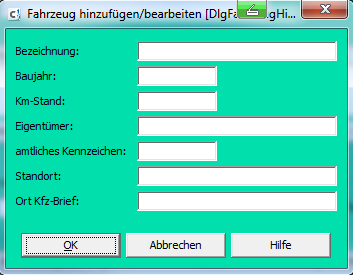
\includegraphics[scale=0.9]{img/FahrzeugAnlegenBearbeiten_Dialog.PNG}
  \caption{neuer Dialog für die Eingabe von Fahrzeugen.}
    \caption*{\textbf{Quelle:} eigene Darstellung}
  \label{fig:fahrzeugAnlegenBearbeitenDialog}
\end{figure}
Durch die Tabelle \glqq Fahrzeug\grqq{} (vgl. \ref{fig:neuerDialog}) bekommt man schnell einen Überblick über alle angelegten Fahrzeuge. Diese lassen sich auch nach der Anlage ohne großen Aufwand noch bearbeiten oder auch wieder löschen. Die neue Lösung verhindert inkonsistente und falsche Daten. Zudem werden Informationen bei der Eingabe, aufgrund der vorgegebenen Eingabestruktur, nicht so schnell vergessen. Dies folgt auch dem Grundsatz \glqq Recognition rather than recall\grqq{} von Jakob Nielsen.

Die letzte Sektion \glqq B. Forderungen, Guthaben und ähnliche Rente\grqq{} beinhaltet Informationen über das Einkommen des Schuldners, über mögliche Drittschuldner und über Immobiliar. Durch die Berücksichtigung von Empfehlungen zur Aufgabenangemessenheit (vgl. ISO 9241-110 Kap. 4.2.3) und zu einem minimalistischen Design (vgl. Jakob Nielsen Kap. 4.2.5) konnten hier einige Informationen, im Vergleich zum vorherigen Dialog, entfallen. Im vorherigen Dialog wurden die Informationen in drei getrennten Reitern dargestellt. Dies hatte den Nachteil, dass der Benutzer häufig zwischen den Reitern wechseln musste. Zusätzlich wurden noch eine handvoll weiterer Informationen neben dran angezeigt, die überflüssig waren und das Erscheinungsbild unübersichtlicher gemacht haben. Die neue Oberfläche stellt nur die nötigsten Informationen dar und wirkt damit viel aufgeräumter und übersichtlicher und ist der Aufgabenstellung angepasst.

Grundsätzlich wurde sich bei der Gestaltung des neuen Dialogs an interne (Style)-Richtlinien der IFM gehalten. Darunter fällt, dass es Schaltflächen wie \glqq OK\grqq{} zum Bestätigen bzw. Speichern, \glqq Abbrechen\grqq{} zum Schließen ohne Speichern und \glqq Hilfe\grqq{} zum Öffnen einer internen Dokumentation gibt. Durch die Einhaltung der Standards wird zugleich dem Ziel der Erwartungskonformität aus der ISO 9241-110 Norm  zu gearbeitet. Eine weiterer Richtlinie der IFM besagt, dass Eingabefelder, Comboboxen und Buttons vorgegebene Abmessungen in der Höhe besitzen und Dialoge auch bei 125\% Anzeigevergrößerung ohne Fehler oder Einschränkungen angezeigt werden. Die Vergrößerung der Anzeige, soll Sachbearbeitern mit eingeschränktem Sehvermögen das Arbeiten erleichtern.

Mit dem Abschluss der Entwicklungsphase geht eine finale Gestaltungslösung als neuer Vermögensverzeichnis Dialog produktiv. Dieser soll für den weiteren Verlauf des Projekts genutzt werden. Dazu soll als nächster Schritt eine vergleichende Evaluation zwischen dem alten und dem neuen Dialog, auf der Basis empirischer Daten, durchgeführt werden.

%%%%%%%%%%%%%%%%%%%%%%%%%%%%%%%%%%%%%%%%%%%%%%%%%%%%%%%%%%%%%%%%%%%%%%%%%%%%

